\documentclass[slovene,11pt,a4paper]{article}

\usepackage[margin=1.5cm,bottom=3cm,foot=1.5cm]{geometry}
\usepackage{amsmath}
\usepackage{booktabs}
\usepackage{float}
\usepackage{graphicx}
\usepackage{changepage}
\usepackage{subcaption}
\usepackage{multirow}
\usepackage{blindtext}
\usepackage{hyperref}
\usepackage[version=4]{mhchem}
\usepackage[slovene]{babel}

\pagenumbering{gobble}

\begin{document}

\title{1. naloga \\ Modeliranje 1-D porazdelitev: Razpadi Higgsovega bozona}
\author{Tadej Lozej 28242023}
\maketitle

\begin{center}
Praktikum strojnega učenja v fiziki \\
\bigskip
Predavatelj: red. prof. dr. Borut Paul Kerševan \\
Asistent: Jan Gavranovič
\end{center}

\newpage

\tableofcontents

\newpage

\pagenumbering{arabic}

\section{Uvod}

Iskanje signala v veliki količini podatkov je velik izziv, saj so le-ti praviloma težko ločljivi od dominantnih procesov ozadja. Pomembno je, da kinematično porazdelitev ozadja čim bolj natančno opišemo, da ga lahko nato odštejemo od podatkov. Na ta način nam nato ostane le možen iskani signal.

Pri opisu procesov ozadja si pomagamo z regresijo ('fitom', parametrizacijo) kinematičnih porazdelitev, ki nas zanimajo. Postopek regresije ozadja izhaja ali iz simuliranih porazdelitev ali iz predpostavljenih funkcijskih oblik, ki jih poskušamo prilagoditi podatkom v kinematičnem območju porazdelitve, kjer signala ne pričakujemo in jih nato ekstrapoliramo v signalno območje.

Metode regresije so danes pomemben element metod strojnega učenja, kjer poskušamo iz omenjene količine podatkov izvleči čim več informacij o samem procesu.

V dani nalogi bomo obravnavali meritev eksperimenta ATLAS, kjer so iskali redek razpad Higgsovega bozona v dva miona $(H \rightarrow \mu^+ \mu^-)$. Ogledali si bomo kinematično porazdelitev dogodkov po rekonstruirani invariantni masi dveh izbranih mionov $(m_{\mu\mu})$. Glavni proces ozdaja je razpad šibkega bozona $(Z \rightarrow \mu^+ \mu^-)$, ki prispeva
resonančno porazdelitev z vrhom pri $m_Z = 91 \, \text{GeV}$, kjer pa se rep invariantne mase razširi tudi precej nad maso Higgsovega bozona $m_H = 125 \, \text{GeV}$. Ta proces ozadja je za več velikostnih redov dogodkov večji, kot jih pričakujemo iz signalnega razpada Higgsovega bozona. K ozadju v manjši meri prispevajo tudi drugi procesi.

Za to nalogo so na razpolago simulirani in izmerjeni dogodki kolaboracije ATLAS. V primeru simulacij so dogodki uteženi tako, da je vsota uteži enaka pričakovani vrednosti števila izmerjenih dogodkov za vključene procese $(\sum wt = N_{proc})$. Celotna statistična napaka je $\sigma = \sqrt{\sum wt^2}$. To za simulacijo pomeni, da napaka ni Poissonova.

Signal lahko za potrebe določitve ozadja omejimo na primer na območje [$120 \, \text{Gev}$, $130 \, \text{GeV}$]. Na voljo imamo cel šop metod za ustrezno določitev ozadja

\begin{itemize}
    \item Polinom dovolj nizkega reda.
    \item Bolj sofisticirane funkcije (mBW)
    \item Support Vectom Machines (SVM) metode z različnimi jedri in regulizatorji
    \item Uporabimo gaussovske procese (Gaussian Process Regression, GPR) z različnimi jedri
    \item  Uporabimo dekompozicijo na ortogonalne polinome
\end{itemize}

Za parametrizacijo signala se tipično uporabi Crystal Ball (CB) funkcija.

\section{Navodila in usmeritve}

\begin{enumerate}
    \item Iz surovih podatkov zgeneriraj svoje histograme s pomočjo predpripravljene skripte \texttt{create\_histograms.py}, pri kateri lahko spreminjaš število predalov in $m_{\mu \mu}$ interval, ki ga boš opazoval/-a. Histogrami (mejne in sredinske $x$ vrednosti predalov, vrednosti in napake) se shranijo v formatu \texttt{.npz}.
    \item Ko imaš zgenerirane svoje histograme, jih lahko izrišeš s pomočjo skripte \texttt{visualize\_data.py} (ustrezno s točko spremeni ime datotek, ki jih nalagaš).
    \item Preveri, če imaš napake res pravilno upoštevane. Lahko jih namenoma pokvariš, in ponoviš prva dva koraka, da vidiš vpliv.
    \item Da se spoznaš z osnovnim fitanjem, najprej zgladi histogram simuliranega ozadja s pomočjo preprostejših matematičnih funkcij in nadaljuj do različnih teoretično podkrepljenih nastavkov. Dobiš funkcijo $m(x_k)$.
    \item Prilagodi funkcijo CB histogramu simuliranega signala, pri čemer upoštevaj še dodatni normalizacijski faktor. Dobiš funkcijo $s(x_k)$.
    \item Ker simulacija ozadja ni vedno najboljša, se po navadi za oceno ozadja vzame izmerjene podatke, pri čemer pa je potrebno izključiti območje, kjer pričakujemo signal. Prilagodi torej funkcijo histogramu podatkov, da dobiš dobro oceno za ozadje in pri tem pazi, da pri fitu ne upoštevaš območja okrog mase Higgsovega bozona. Dobiš funkcijo $b(x_k)$.
    \item Od podatkov odštej čimbolj zglajeno ozadje, ki si ga dobil v prejšnji točki, da dobiš ekstrahiran signal $y(x_k)$.
    \item Na ekstrahiran signal fitaj CB funkcijo s prostimi parametri, ki si jih dobil v točki 5. tako, da ji v resnici prilagodiš le nov normalizacijski faktor $\alpha_{norm} \cdot s(x_k)$.
    \item Ker je izmerjenega signala še zelo malo, predlagamo, da postopek najprej narediš z umetno napihnjenim signalom - le tega množi s faktorjem $\gamma = 100$ in ga dodaj podatkom $d_{new}(x_k) = d(x_k) + \gamma s(x_k)$. Ker bo ta signal na ta način lepo izstopal iz ozadja, ga boš lažje izluščil.
\end{enumerate}

\section{Podatki}

Za začetek si oglejmo realne podatke, ki jih imamo v datoteki \texttt{data.h5}. V tej datoteki imamo na voljo 106148612 dogodkov. Na sliki \ref{fig:data} imamo histogram z 100 000 predalčki med minimalno in maksimalno vrednostjo invariantne mase dogodkov. Na levi osi vidimo absolutno število dogodkov pri določenem predalčku invariantne mase na desni osi pa relativno število dogodkov. Na manjše je prikazan tuki histogram v široki okolici mase Higgsovega bozona $m_H = 125 \, \text{GeV}$. Vidimo visok vrh pri razpadu šibkega bozona pri invariantni masi $m_Z = 91 \, \text{GeV}$. Vrh Higgsovega bozona na histogramu ni niti viden.

\begin{figure}[h!]
    \centering
    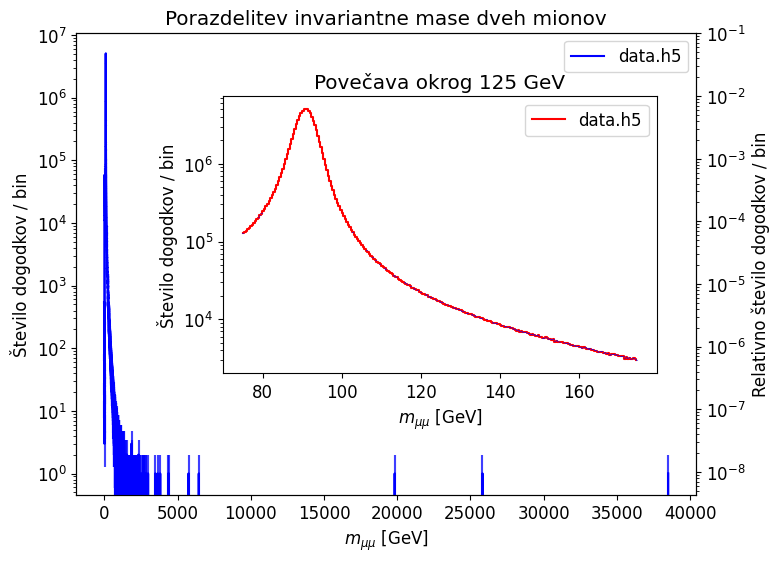
\includegraphics[width=0.8\linewidth]{imgs/data.png}
    \caption{Histogam porazdelitve invariantne mase dveh mionov iz datoteke \texttt{data.h5}. Na levi osi je absolutna skala na desni pa relativna. Na manjše je prikazan histogram v okolici invariantne mase Higgsovega bozona.}
    \label{fig:data}
\end{figure}

\begin{figure}[h!]
    \centering
    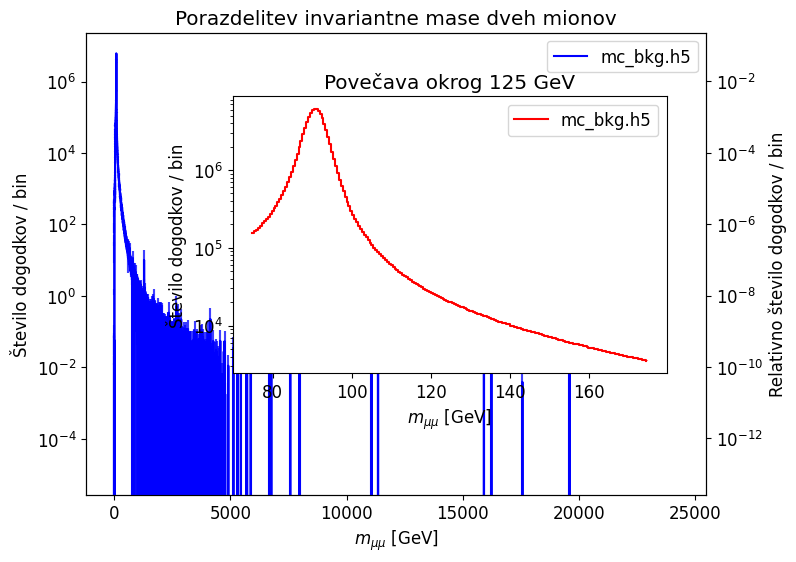
\includegraphics[width=0.8\linewidth]{imgs/mc_bkg.png}
    \caption{Histogam porazdelitve invariantne mase dveh mionov iz datoteke \texttt{mc\_bkg.h5}. Na levi osi je absolutna skala na desni pa relativna. Na manjše je prikazan histogram v okolici invariantne mase Higgsovega bozona.}
    \label{fig:mc_bkg}
\end{figure}

\begin{figure}[h!]
    \centering
    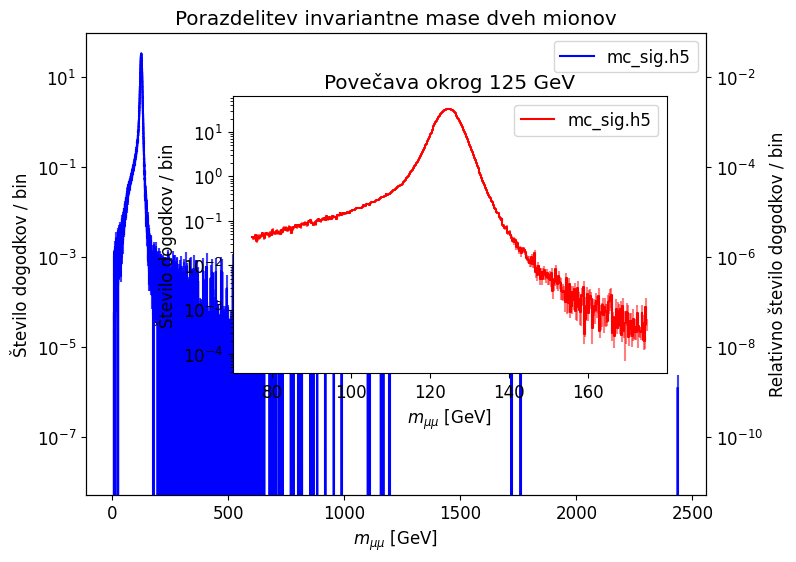
\includegraphics[width=0.8\linewidth]{imgs/mc_sig.png}
    \caption{Histogam porazdelitve invariantne mase dveh mionov iz datoteke \texttt{mc\_sig.h5}. Na levi osi je absolutna skala na desni pa relativna. Na manjše je prikazan histogram v okolici invariantne mase Higgsovega bozona.}
    \label{fig:mc_sig}
\end{figure}

Na sliki \ref{fig:mc_bkg} je prikazana porazdelitev invariantne mase dveh mionov iz datoteke \texttt{mc\_bkg.h5}. Na voljo imamo 311281902 dogodkov. Razporedil sem jih v 50 000 enako velikih predalčkov med minimalno in maksimalno invariantno maso. Te podatke so pridobili s pomočjo Monte Carlo simulacije. Simulirali so zgolj ozadje procesa. Vsak dogodek je utežen in zato smo pri risanju histograma morali biti na to pozorni in dogodek šteti sladno z njegovo utežjo. Kot na prejšnjem grafu sta tudi tukaj leva in desna os grafa absolutno ter relativno število dogodkov. Vidimo, da je histogram na prvi pogled precej podoben. Na manjše imamo kot prej prikazan histogram v širši okolici invariantne mase Higgsovega bozona.

Na sliki \ref{fig:mc_sig} lahko vidimo porazdelitev invariantne mase dveh mionov iz datoteke \texttt{mc\_sig.h5}. Na voljo imamo 5498243 dogodkov. Razporedil sem jih v 10 000 enako velikih predalčkov med minimalno in maksimalno invariantno maso. Te podatke so pridobili s pomočjo Monte Carlo simulacije. Simulirali so zgolj signal procesa t. j. razpad Higgsovega bozona. Enako kot prej imamo na levi ter desni absolutno ter relativno preštete dogodke v predalčkih invariantnih mas. Vidimo, da je tovrstnih dogodkov precej malo. Na manjšem grafu z rdečo vidimo histogram v širši okolici invariantne mase Higgsovega bozona.

Na sliki \ref{fig:my_hist} je prikazan histogram generiran s funkcijo \texttt{make\_histograms} in narisan s funkcijo \linebreak \texttt{visualize\_histograms}. Vidimo porazdelitev invariantne mase dveh mionov v merjenih podatkih (Data), simuliranem ozadju (Ozadje) ter simuliranem signalu (Signal). Na spodnjem histogramu lahko vidimo razmerje med številom merjenih dogodkov ter simuliranih dogodkov v ozadju.

\begin{figure}[h!]
    \centering
    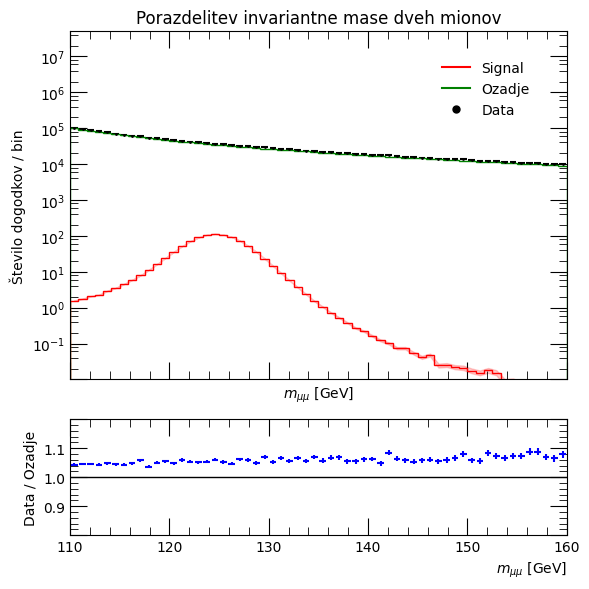
\includegraphics[width=0.8\linewidth]{imgs/my_hist.png}
    \caption{Histogam porazdelitve invariantne mase dveh mionov izvseh treh datotek. Spodaj je prikazano razmerje med merjenimi podatki ter simuliranim ozadjem.}
    \label{fig:my_hist}
\end{figure}

\section{Glajenje ozadja z analitičnimi funkcijami}

Cilj naloge je odšteti ozadje meritvam in izluščiti signal. Za ta proces bo potrebno dobro modelirati ozadje. V tem delu naloge bomo ozadje poskušali modelirati z analitičnimi funkcijami

\begin{itemize}
    \item Polinomi različnih stopenj: $a_0 + a_1 x + a_2 x^2 + a_3 x^3 + ...$
    \item Potenčna funkcija: $ax^b$
    \item Eksponentna funkcija: $a_1 \exp(-b_1 x) + a_2 \exp(-b_2 x)$
    \item Dijet funkcija: $a(1-x^d)^c x^{b_1 + b_2 \ln(x)}$
    \item Eksponent polinoma: $a \exp(b_1 x + b_2 x^2 + b_3 x^3)$
    \item CMS funkcija: $\exp(a_2 m + a_3 m^2) / ((m-m_Z)^{a_1} + (0.5g_Z)^{a_1})$,
\end{itemize}
kjer je $x$ število dogodkov, ki se pojavijo v histogramu, $m_Z$ in $g_Z$ pa lastnosti Z bozona. Vse ostalo so prosti parametri.

\subsection{Simulirano ozadje}

Osredotočimo se na simulirano ozadje iz datoteke \texttt{mc\_sig.h5}. Z različnimi funkcijami bomo poskusili čimbolje opisati ozadje na intervalu prikazanem na sliki \ref{fig:my_hist}. Za začetek si na sliki \ref{fig:polinomi} oglejmo različne fite polinomov na simulirano ozadje. Z različnimi barvami so  prikazane različne stopnje polinomov. V legendi poleg tega piše tudi vrednost reduciranega chi kvadrata fita $\chi^2_{red}$. To je navaden $\chi^2$ deljen s prostorskimi stopnjami modela $\nu = N-p$, kjer je $N$ število izmerjenih točk ter $p$ število prostih parametrov modela.To vrednost povezujemo z kvaliteto modela. Če je vrednost enaka 1 pomeni, da model precej dobro opiše obnašanje in tudi ni preveč prilagojen na konkreten primer. Če je vrednost manjša od 1 je bodisi naš model preveč natančen ali pa so napake meritev podcenjene. Če je vrednost večja kot 1 pa bodisi naš model ni preveč dober bodisi so napake precenjene. Vidimo, da v primeru polinomov najmanjšo vrednost zavzame polinom s stopnjo 5.

\begin{figure}[h!]
    \centering
    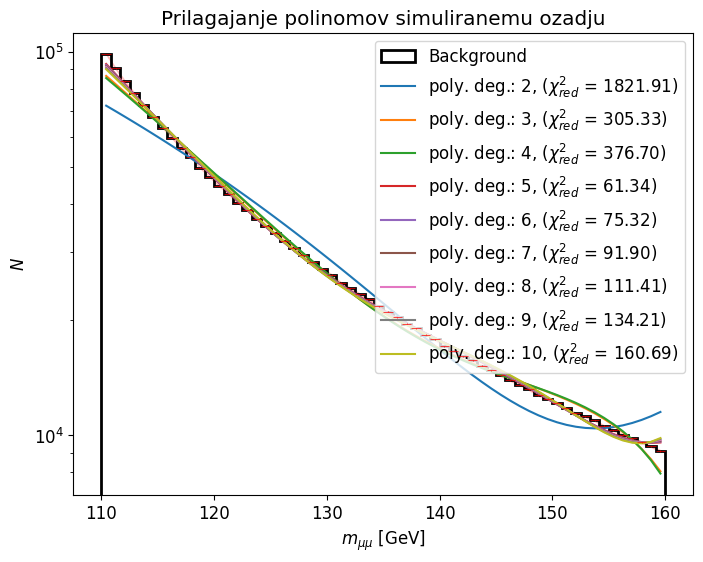
\includegraphics[width=0.8\linewidth]{imgs/polinomi.png}
    \caption{Polinomi različnih stopenj prilagojeni simuliranemu ozadju. V legendi imamo za vsak model podano tudi vrednost reduciranega $\chi^2_{red}$.}
    \label{fig:polinomi}
\end{figure}

Naprej si poglejmo še preostale analitične funkcije. Na sliki \ref{fig:modeli} lahko vidimo preostale omenjene modelske funkcije. Eksponentna in eksponent polinoma imata zelo majhno vrednost $\chi^2_{red}$. Tudi bolj teoretično podkovana funkcija CMS se precej lepo prilagaja ozadju. Program je imel težave pri ocenjevanju napak parametrov Dijet funkcije in zato tudi ni znal izračunati pripadajoče vrednosti $\chi^2_{red}$.

\begin{figure}[h!]
    \centering
    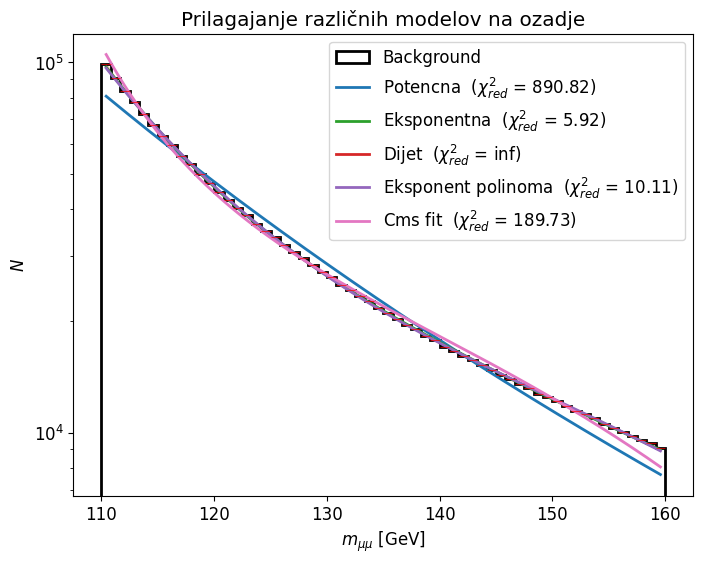
\includegraphics[width=0.8\linewidth]{imgs/modeli.png}
    \caption{Različne modelske funkcije prilagojene simuliranemu ozadju. V legendi imamo za vsak model podano tudi vrednost reduciranega $\chi^2_{red}$.}
    \label{fig:modeli}
\end{figure}

\begin{figure}[h!]
    \centering
    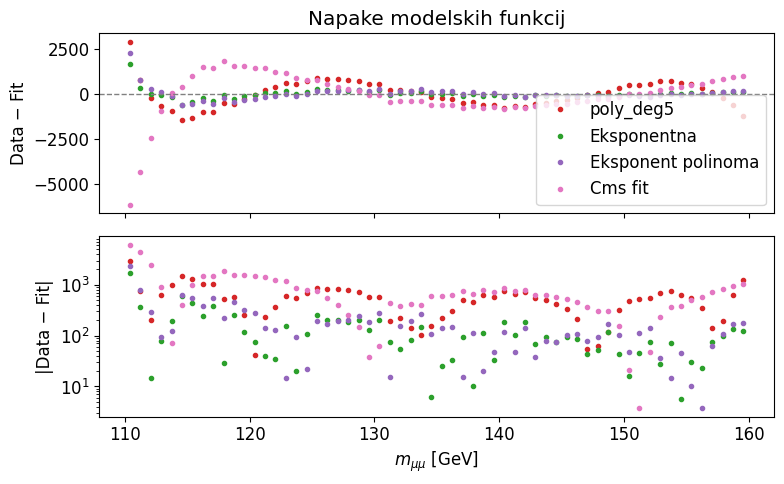
\includegraphics[width=0.8\linewidth]{imgs/najboljsi_modeli.png}
    \caption{Napake najboljših modelskih funkcij. Zgoraj v linearni skali spodaj pa v logaritemski.}
    \label{fig:najboljsi_modeli}
\end{figure}

Na sliki \ref{fig:najboljsi_modeli} lahko vidimo napake najboljših modelov. Vidimo, da se v območju mase Higgsovega bozona najbolje prilegata eksponent in eksponent polinoma. Nevem pa, če bi temu lahko rekli dobro prileganje... 

\subsection{Simuliran signal}

Za vajo lahko poskusimo prilagoditi Crystal Ball funkcijo simuliranemu signalu iz datoteke \texttt{mc\_sig.h5}. Na sliki \ref{fig:CB} lahko vidimo Crystal Ball funkcijo prilagojeno simuliranemu signalu. Spodaj lahko vidimo tudi njeno odstopanje. Prilagojena funkcija se precej dobro ujema s podatki.

\begin{figure}[h!]
    \centering
    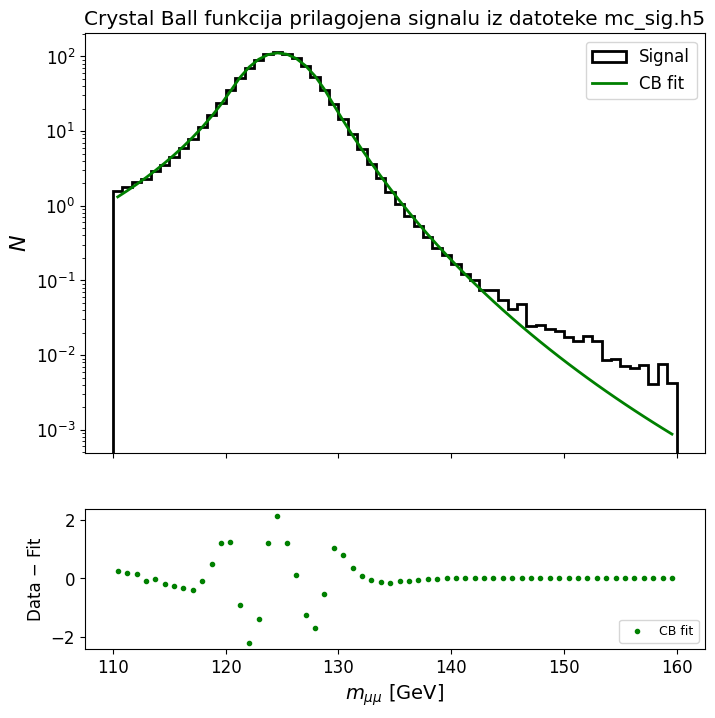
\includegraphics[width=0.8\linewidth]{imgs/CB.png}
    \caption{Crystal Ball funkcija prilagojena simuliranemu signalu. Sporaj je prikazano odstopanje fita od podatkov.}
    \label{fig:CB}
\end{figure}

\subsection{Dejanski in napihnjeni podatki}

Poglejmo si sedaj še prilagajanje funkcij dejanskih podatkom iz datoteke \texttt{data.h5}. Pazizi moramo, da ne upoštevamo območja signala. Na sliki \ref{fig:BrezSignala} lahko vidimo podatke z izrezanim območjem v okolici vrha signala. Območje smo odrezali med invariantno maso $120$ ter $130 \, \text{GeV}$.

Na sliki \ref{fig:RazlicniPodatki} imamo prikazane različne podatke. Z črnimi pikami vidimo podatke iz katerih smo odvzeli signalno območje. Tem bomo prilagajali naše modelske funkcije. Zelen histogram prikazuje vse podatke. Rdeč histogram prikazuje podatke iz simulacije signala pomnožene s faktorjem $\gamma = 100$. Moder histogram prikazuje podatke katerim smo prišteli umetno napihnjen simuliran signal. Tako je moder histogram v resnici zeles s prištetim rdečim. Tem podatkom bomo rekli Asimov podatki.

\begin{figure}[h!]
    \centering
    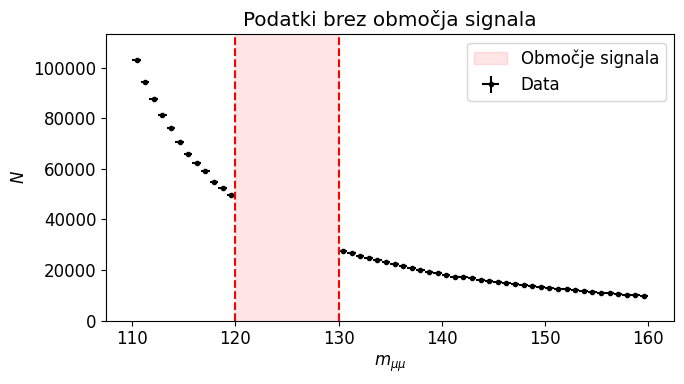
\includegraphics[width=0.8\linewidth]{imgs/BrezSignala.png}
    \caption{Dejanski podatki brez območja signala.}
    \label{fig:BrezSignala}
\end{figure}

\begin{figure}[h!]
    \centering
    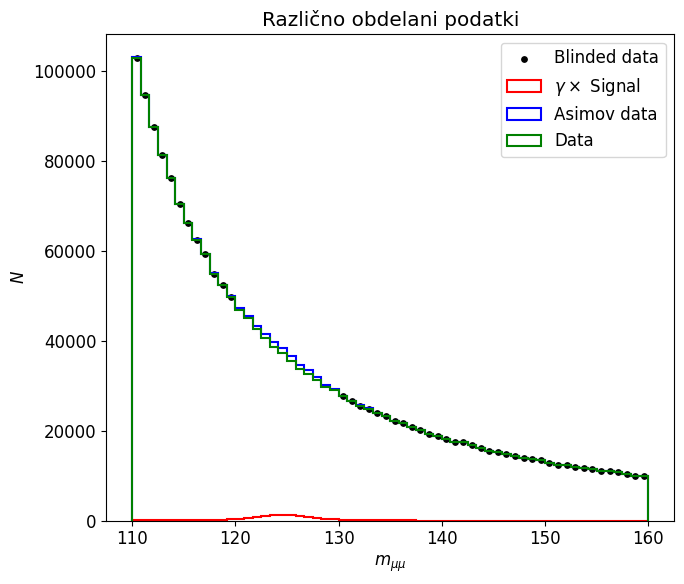
\includegraphics[width=0.8\linewidth]{imgs/RazlicniPodatki.png}
    \caption{Različni podatki. Z črnimi pikami so prikazani podatki brez območja signala. Tem bomo prilagajali funkcije. Nato so pa po vrsti Napihnjen signal, Asimov podatki ter podatki.}
    \label{fig:RazlicniPodatki}
\end{figure}

Na naslednjih dveh slikah \ref{fig:IzluscenSignalData} in \ref{fig:IzluscenSignalAsimovData} lahko vidimo funkcije ozadja narisane čez podatke ter napšihnjene podatke ter izluščen signal iz podatkov ter napihnjenih podatkov. Kot pričakovano smo več signala dobili iz podatkov z napihnjenim signalom. Izluščenim signalom sem se trudil prilagoditi CrystallBall funkcijo ampak žal neuspešno.

\begin{figure}[h!]
    \centering
    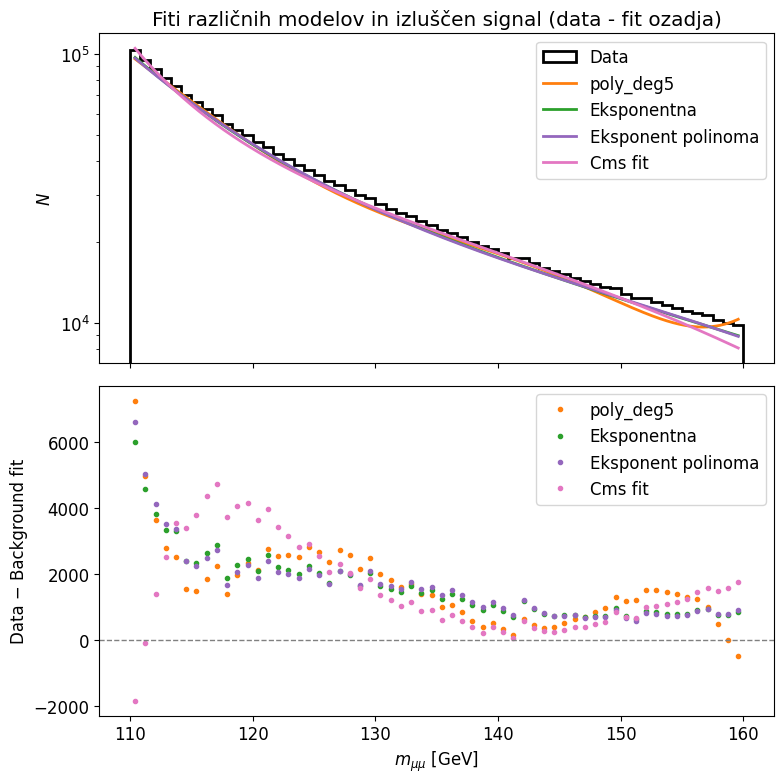
\includegraphics[width=0.8\linewidth]{imgs/IzluscenSignalData.png}
    \caption{Funkcije prilagojene ozadju narisena čez podatke zgoraj ter izluščen signal spodaj.}
    \label{fig:IzluscenSignalData}
\end{figure}

\newpage

\begin{figure}[h!]
    \centering
    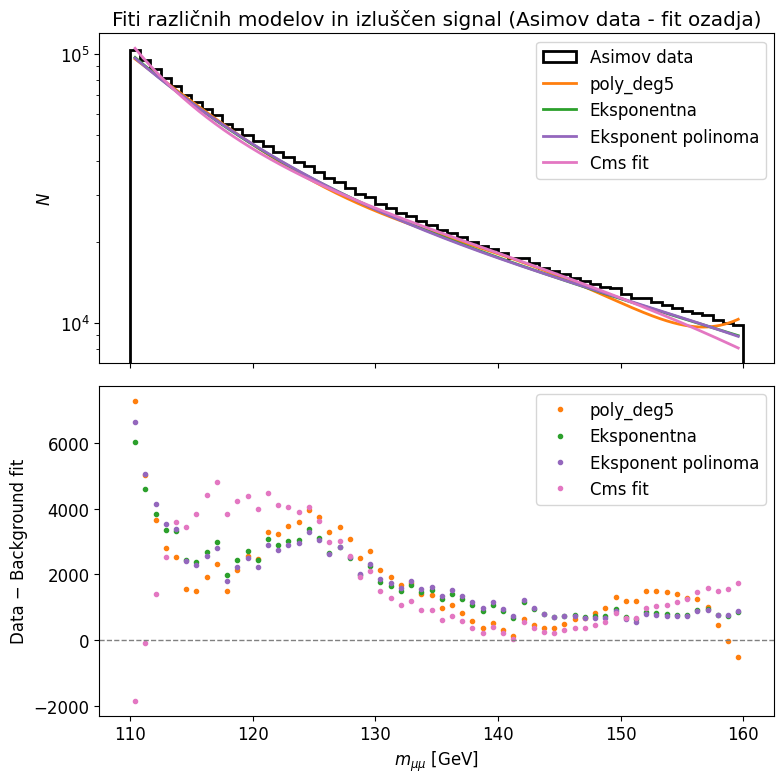
\includegraphics[width=0.8\linewidth]{imgs/IzluscenSignalAsimovData.png}
    \caption{Funkcije prilagojene ozadju narisena čez napihnjene podatke zgoraj ter izluščen signal spodaj.}
    \label{fig:IzluscenSignalAsimovData}
\end{figure}

\section{Glajenje ozadja z Gaussovskimi procesi}

\end{document}